\documentclass{nudtproposal}
% --- preamble --- %
% --- preamble --- %
\usepackage{amsmath}
\usepackage{silence}
\WarningsOff

\usepackage{listings}
\lstset{
    basicstyle          =   \sffamily,          % 基本代码风格
    keywordstyle        =   \bfseries,          % 关键字风格
    commentstyle        =   \rmfamily\itshape,  % 注释的风格,斜体
    stringstyle         =   \ttfamily,  % 字符串风格
    flexiblecolumns,                % 别问为什么,加上这个
    % numbers             =   left,   % 行号的位置在左边
    showspaces          =   false,  % 是否显示空格,显示了有点乱,所以不现实了
    % numberstyle         =   \normalsize\ttfamily,    % 行号的样式,小五号,tt等宽字体
    showstringspaces    =   false,
    captionpos          =   t,      % 这段代码的名字所呈现的位置,t指的是top上面
    frame               =   lrtb,   % 显示边框
}

\lstdefinestyle{texstyle}{
    language        =   tex, % 语言
    basicstyle      =   \normalsize\ttfamily,
    % numberstyle     =   \normalsize\ttfamily,
    keywordstyle    =   \color{blue},
    keywordstyle    =   [2] \color{teal},
    stringstyle     =   \color{magenta},
    commentstyle    =   \color{red}\ttfamily,
    breaklines      =   true,   % 自动换行,建议不要写太长的行
    columns         =   fixed,  % 如果不加这一句,字间距就不固定,很丑,必须加
    basewidth       =   0.5em,
    morekeywords    =   {section,mdframed,label,hspace,begin,end}
}

\usepackage{lipsum}
\usepackage{zhlipsum}
\usepackage{lscape}
\addbibresource{ref/refs.bib}
% --- personal information --- %
\degree{硕士} % 学位:硕士,博士
\confidentiality{公开} % 密级:公开,秘密,机密或者绝密
\papernumber{2411010xx} % 编号
\title{国防科技大学研究生} % 标题第1行
\subtitle{学位论文开题报告} % 标题第2行
\author{张同学} % 作者
\authorid{2301xxxx} % 学号
\advisor{xxx} % 导师
\advisortitle{教~~~~授} % 职称
\degreetype{理学} % 学位类别
\major{数~~~~学} % 一级学科
\field{xxx} % 研究方向
\institute{理学院}% 学院
\year{2024}
\month{12}
\day{1}
% \zhdate{二〇二四年十一月} % 中文日期

\begin{document}
\maketitle
\BeforeBeginEnvironment{tabular}{\zihao{5}}
\section{学位论文选题的立论依据}\label{sec:background}
\subsection{课题来源}
自拟。

\subsection{基本概念}
\subsubsection{插入图表}
下面来看一个图片实例:
\begin{figure}[htbp]
	\centering
	
\includegraphics[width = 2in]{image/logo.pdf}
	\caption{nudtproposal的logo}
	\label{fig:nudt-proposal}
\end{figure}

如果要把编号的两个图形并排,那么小页(minipage)就非常有用了,可以分别参考\cref{fig:parallel1}和\cref{fig:parallel2}。
\begin{figure}[htb]
\begin{minipage}{0.48\textwidth}
  \centering
  
\includegraphics[height=1.2cm]{image/xhh.eps}
  \caption{并排第一个图}
  \label{fig:parallel1}
\end{minipage}\hfill
\begin{minipage}{0.48\textwidth}
  \centering
  
\includegraphics[height=1.2cm]{image/xhh.eps}
  \caption{并排第二个图}
  \label{fig:parallel2}
\end{minipage}
\end{figure}

若子图共用一个计数器见\cref{fig:big1},它包含两个小图,分别是\cref{fig:subfig1}
和\cref{fig:subfig2}。这里推荐使用\verb|\subfloat|,{\bf 不要再用}
\verb|\subfigure|和\verb|\subtable|。
\begin{figure}[htb]
  \centering%
  \subfloat[第一个小图形]{%
    \label{fig:subfig1}
    
\includegraphics[height=1.56cm]{image/xh.eps}}\hspace{4em}%
  \subfloat[第二个小图形]{%
    \label{fig:subfig2}
    
\includegraphics[height=1.56cm]{image/xhh.eps}}
  \caption{包含子图形的大图形}
  \label{fig:big1}
\end{figure}

下面来看一个表格实例:
\begin{table}[htb]
  \centering
  \begin{minipage}[t]{0.8\linewidth}
  \caption{模板文件}
  \label{tab:template-files}
    \begin{tabular*}{\linewidth}{lp{8cm}}
      \toprule[1.5pt]
      {\hei 文件名} & {\hei 描述} \\
      \midrule[1pt]
      mian.tex & 主程序\footnote{表格中的脚注} \\
      nudtpaper.cls & 模板类文件\footnote{再来一个}。\\
      \bottomrule[1.5pt]
    \end{tabular*}
  \end{minipage}
\end{table}

浮动体的并排放置一般有两种情况:1)二者没有关系,为两个独立的浮动体;2)二者隶属于同一个浮动体。对表格来说并排表格既可以像\cref{tab:parallel1}、\cref{tab:parallel2}使用小页环境,也可以如\cref{tab:subtable}使用子表格来做。

\begin{table}[htb]
\centering\noindent
\begin{minipage}{0.45\textwidth}
	\centering
	\caption{第一个并排子表格}
	\label{tab:parallel1}
	\begin{tabular}{p{2cm}p{2cm}}
		\toprule[1.5pt]
		111 & 222 \\\midrule[1pt]
		222 & 333 \\\bottomrule[1.5pt]
	\end{tabular}
\end{minipage}
\begin{minipage}{0.45\textwidth}
	\centering
	\caption{第二个并排子表格}
	\label{tab:parallel2}
	\begin{tabular}{p{2cm}p{2cm}}
		\toprule[1.5pt]
		111 & 222 \\\midrule[1pt]
		222 & 333 \\\bottomrule[1.5pt]
	\end{tabular}
	\end{minipage}
\end{table}

\begin{table}[htb]
	\centering
	\caption{并排子表格}
	\label{tab:subtable}
	\subfloat[第一个子表格]{
	\begin{tabular}{p{2cm}p{2cm}}
		\toprule[1.5pt]
		111 & 222 \\\midrule[1pt]
		222 & 333 \\\bottomrule[1.5pt]
	\end{tabular}
	}\hskip2cm
	\subfloat[第二个子表格]{
	\begin{tabular}{p{2cm}p{2cm}}
		\toprule[1.5pt]
		111 & 222 \\\midrule[1pt]
		222 & 333 \\\bottomrule[1.5pt]
	\end{tabular}
	}
\end{table}

\subsubsection{插入公式}
贝叶斯公式如式~(\ref{eq:bayes}),其中$p(y|\boldsymbol{x})$为后验;$p(\boldsymbol{x})$为先验;分母$p(\boldsymbol{x})$ 为归一化因子。
\begin{equation}\label{eq:bayes}
	p(y|\boldsymbol{x}) = \frac{p(\boldsymbol{x},y)}{p(\boldsymbol{x})}=
	\frac{p(\boldsymbol{x}|y)p(y)}{p(\boldsymbol{x})}
\end{equation}

再看\cref{eq:split}:
\begin{equation}\label{eq:split}
	\begin{split}
		C(z) &= [z^n] \biggl[\frac{e^{3/4}}{\sqrt{1-z}} +
		e^{-3/4}(1-z)^{1/2} + \frac{e^{-3/4}}{4}(1-z)^{3/2}
		+ O\Bigl( (1-z)^{5/2}\Bigr)\biggr] \\
		&= \frac{e^{-3/4}}{\sqrt{\pi n}} - \frac{5e^{-3/4}}{8\sqrt{\pi
		n^3}} + \frac{e^{-3/4}}{128 \sqrt{\pi n^5}} +
		O\biggl(\frac{1}{\sqrt{\pi
		n^7}}\biggr)
	\end{split}
\end{equation}


\subsubsection{智能引用}
为了增加体验感,使用 `\verb|\cref|' 命令智能引用,例如\cref{fig:nudt-proposal} 、\cref{tab:template-files}和\cref{eq:bayes},但尽量避免在换行处使用该命令。

\subsection{其他事项}
\subsubsection{破折号}
中文破折号为一个两个字宽垂直居中的直线,输入法直接得到的破折号是两个断开的小短线(——),这看起来不舒服。所以模板中定义了一个破折号的命令  `\verb|\pozhehao|',请看:

厚德博学,强军兴国\hfill \pozhehao{}国防科大校训

\subsection{Iguana\TeX{}}
\begin{figure}[htbp]
	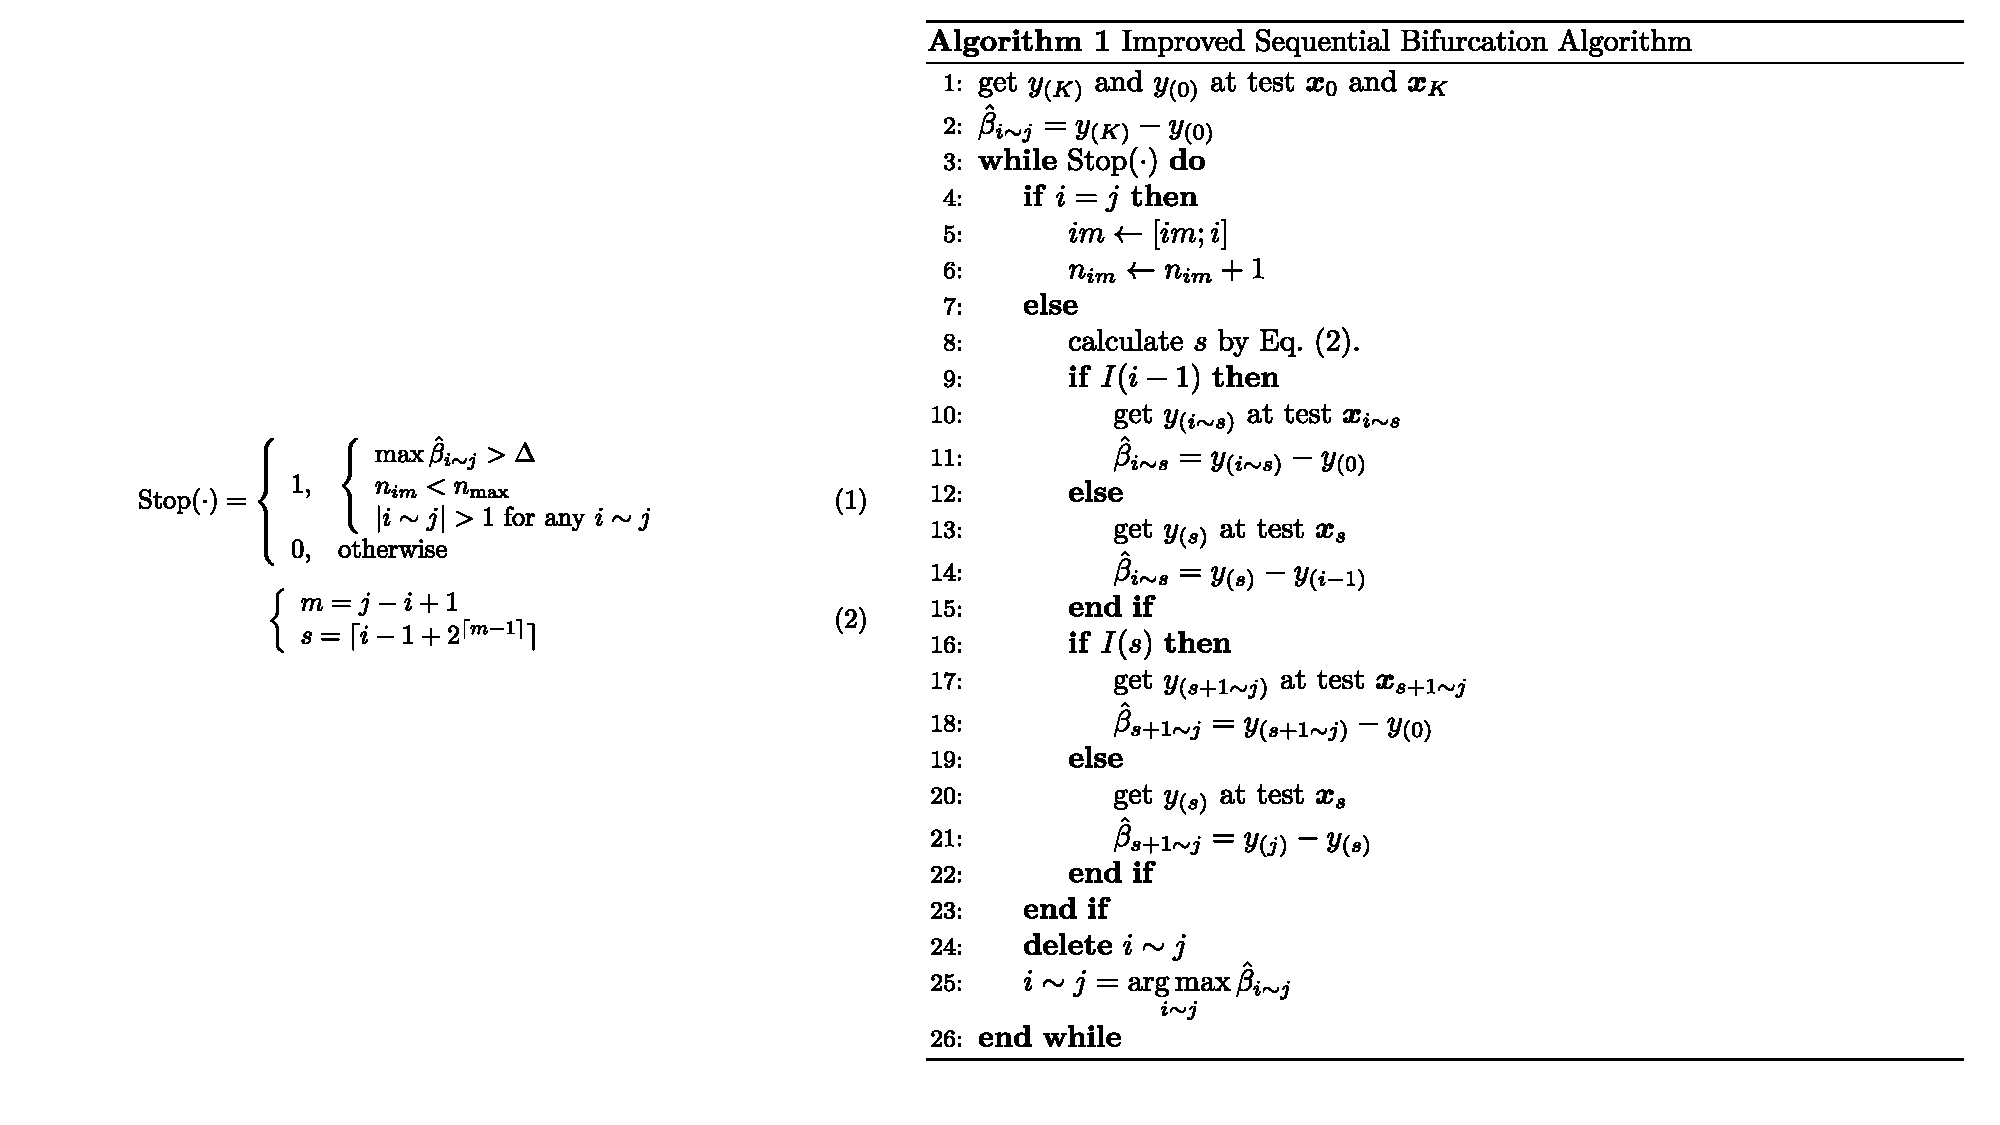
\includegraphics[width=.8\textwidth]{image/IguanaTex.pdf}
	\caption{\href{https://github.com/Jonathan-LeRoux/IguanaTex}{Iguana\TeX{}生成的图片}}
	\label{fig:IguanaTex}
\end{figure}

推荐一个PowerPoint插件 \href{https://github.com/Jonathan-LeRoux/IguanaTex}{Iguana\TeX{}},只要可以用\LaTeX{}生成的文档(甚至是beamer和poster)都可以无损插入到PowerPoint中,\cref{fig:IguanaTex}就是用这个插件成的。

\clearpage
\section{文献综述}\label{sec:referenceSummary}
\subsection{xxx研究综述}
很多文献\cite{almarza1998-student,goosens1994-latex,spivak1988-can,diaozhenren2024-da}……,用来测试`\verb|longtable|'环境换页情况。
\subsection{参考文献表格环境}
第~\ref{sec:references}~节的主要参考文献表格环境参考了文献\parencite{hu_shidong2023-latex}的处理。
\subsection{自己笔记的广告}
给自己写的笔记打个广告\cite{zhangxinhang2023-ren},其他笔记可以见主页\href{https://github.com/Trikim-Zhang}{https://github.com/Trikim-Zhang}。

\clearpage
\section{研究内容}\label{sec:researchContent}

\subsection{研究目标}

\subsection{主要研究内容及拟解决的相关科学问题和技术问题}
	
\subsection{拟采取的研究方法、技术路线、实施方案及可行性分析}

\subsection{预期创新点}

很多内容……

\begin{algorithm}[H]
    \caption{Gauss列主元消元法}
    \label{alg:GaussElim}
    \Input{$[\boldsymbol{A}\,| \boldsymbol{b}]$}
    \Output{$\boldsymbol{x}$}
    $\boldsymbol{Z} = [\boldsymbol{A}\,| \boldsymbol{b}]$\\
    \For{$k = 1\to n-1$}{
        \tcp*[l]{\colorbox{cyan!50}{A}}
        \For{$i = k+1\to n$}{
            \tcp*[l]{\colorbox{cyan!50}{B}}
            $\boldsymbol{Z}[i,:]\gets \boldsymbol{Z}[i,:]-\dfrac{a_{ik}^{(k)}}{a_{kk}^{(k)}}\boldsymbol{Z}[k,:]$
        }
        \tcp*[l]{\colorbox{cyan!50}{C}}
    }
    $\boldsymbol{A} = \boldsymbol{Z}[:,1:n]$\\
    $\boldsymbol{b} = \boldsymbol{Z}[:,n+1]$\\
    \For{$i = n\to 1$}{
        \tcp*[l]{\colorbox{cyan!50}{D}}
        $\boldsymbol{x}[{i}] = \boldsymbol{b}[i]$\\
        $\boldsymbol{x}[{i}] = \boldsymbol{x}[{i}]-\boldsymbol{A}[i,i+1:]\boldsymbol{x}[i+1:]$\\
        $\boldsymbol{x}[i] = \boldsymbol{x}[i]/\boldsymbol{A}[i,i]$
    }
    \Return {$\boldsymbol{x}$}
\end{algorithm}

\clearpage
\section{研究条件}\label{sec:researchCondition}
开展研究应具备的条件及已具备的条件,可能遇到的困难与问题和解决措施。

\clearpage
\section{学位论文工作计划}\label{sec:schedule}
{
\noindent
\begin{slongtable}{| C{0.20\textwidth} | C{0.40\textwidth} | C{0.311\textwidth} |}
  \hline 
	\multicolumn{1}{|c|}{起讫日期} & 	\multicolumn{1}{c}{主要完成研究内容} & 	\multicolumn{1}{|c|}{预期成果} \\
	\hline 
	2017年09月 \par\pozhehao\par 2018年03月  & 基础知识学习 & 完成文献搜集与该方向基本知识储备 \\ 
	\hline 
	2018年04月 \par\pozhehao\par 2018年06月 & 研究点1 &  完成实验 \\ 
	\hline 
	2018年07月 \par\pozhehao\par 2018年08月 & 研究点1 &  发表论文SCI一篇 \\ 
	\hline 
	2018年09月 \par\pozhehao\par 2018年10月 & 研究点2 &  完成实验 \\ 
	\hline 
    2018年11月 \par\pozhehao\par 2018年12月 & 研究点2 &  发表论文EI一篇 \\ 
    \hline 
    2019年01月 \par\pozhehao\par 2019年02月 & 研究点3 &  完成实验 \\ 
    \hline 
    2019年03月 \par\pozhehao\par 2019年04月 & 研究点3 &  发表论文EI一篇 \\ 
    \hline 
    2019年05月 \par\pozhehao\par 2019年06月 & 研究点4 &  完成实验 \\ 
    \hline 
    2019年07月 \par\pozhehao\par 2019年08月 & 研究点4 &  发表论文EI一篇 \\ 
    \hline 
    2019年09月 \par\pozhehao\par 2019年09月 & 研究点5 &  完成实验 \\ 
    \hline 
    2019年10月 \par\pozhehao\par 2019年10月 & 研究点5 &  发表论文EI一篇 \\ 
    \hline 
	2019年11月 \par\pozhehao\par 2020年01月 & 撰写毕业论文 & 完成毕业论文 \\ 
	\hline 
\end{slongtable}
注:每个子阶段不得超过3个月;预期成果中必须包含成果的形式、数量、质量等可考性指标该计划将作为论文研究进展检查的依据。
\indent
}
\clearpage
\section{主要参考文献}\label{sec:references}
\vspace*{-16pt}
\nocite{*}
\printbibtabular[title={~}]
\clearpage
\section{指导教师对开题报告的评语}\label{sec:advisorComments}
(对1-6项逐项予以评价,并着重对国内/外研究现状的了解情况、研究内容的创新性等方面进行评价,最终给出是否满足博士/硕士层次学位论文研究要求的综合评价意见)

课题评价。……

符合硕士研究生开题要求。
\vfill{}\,
\begin{flushright}
    \begin{tabular}{rr}
       导师签字: & \multicolumn{1}{c}{
\includegraphics[width = 5em]{figure/dalei.pdf}} \\[10 mm]
            & 2024年12月20日 \\[30 mm]
    \end{tabular}%
\end{flushright}
%评审意见直接插进来就行,最终版用签字扫描版替代
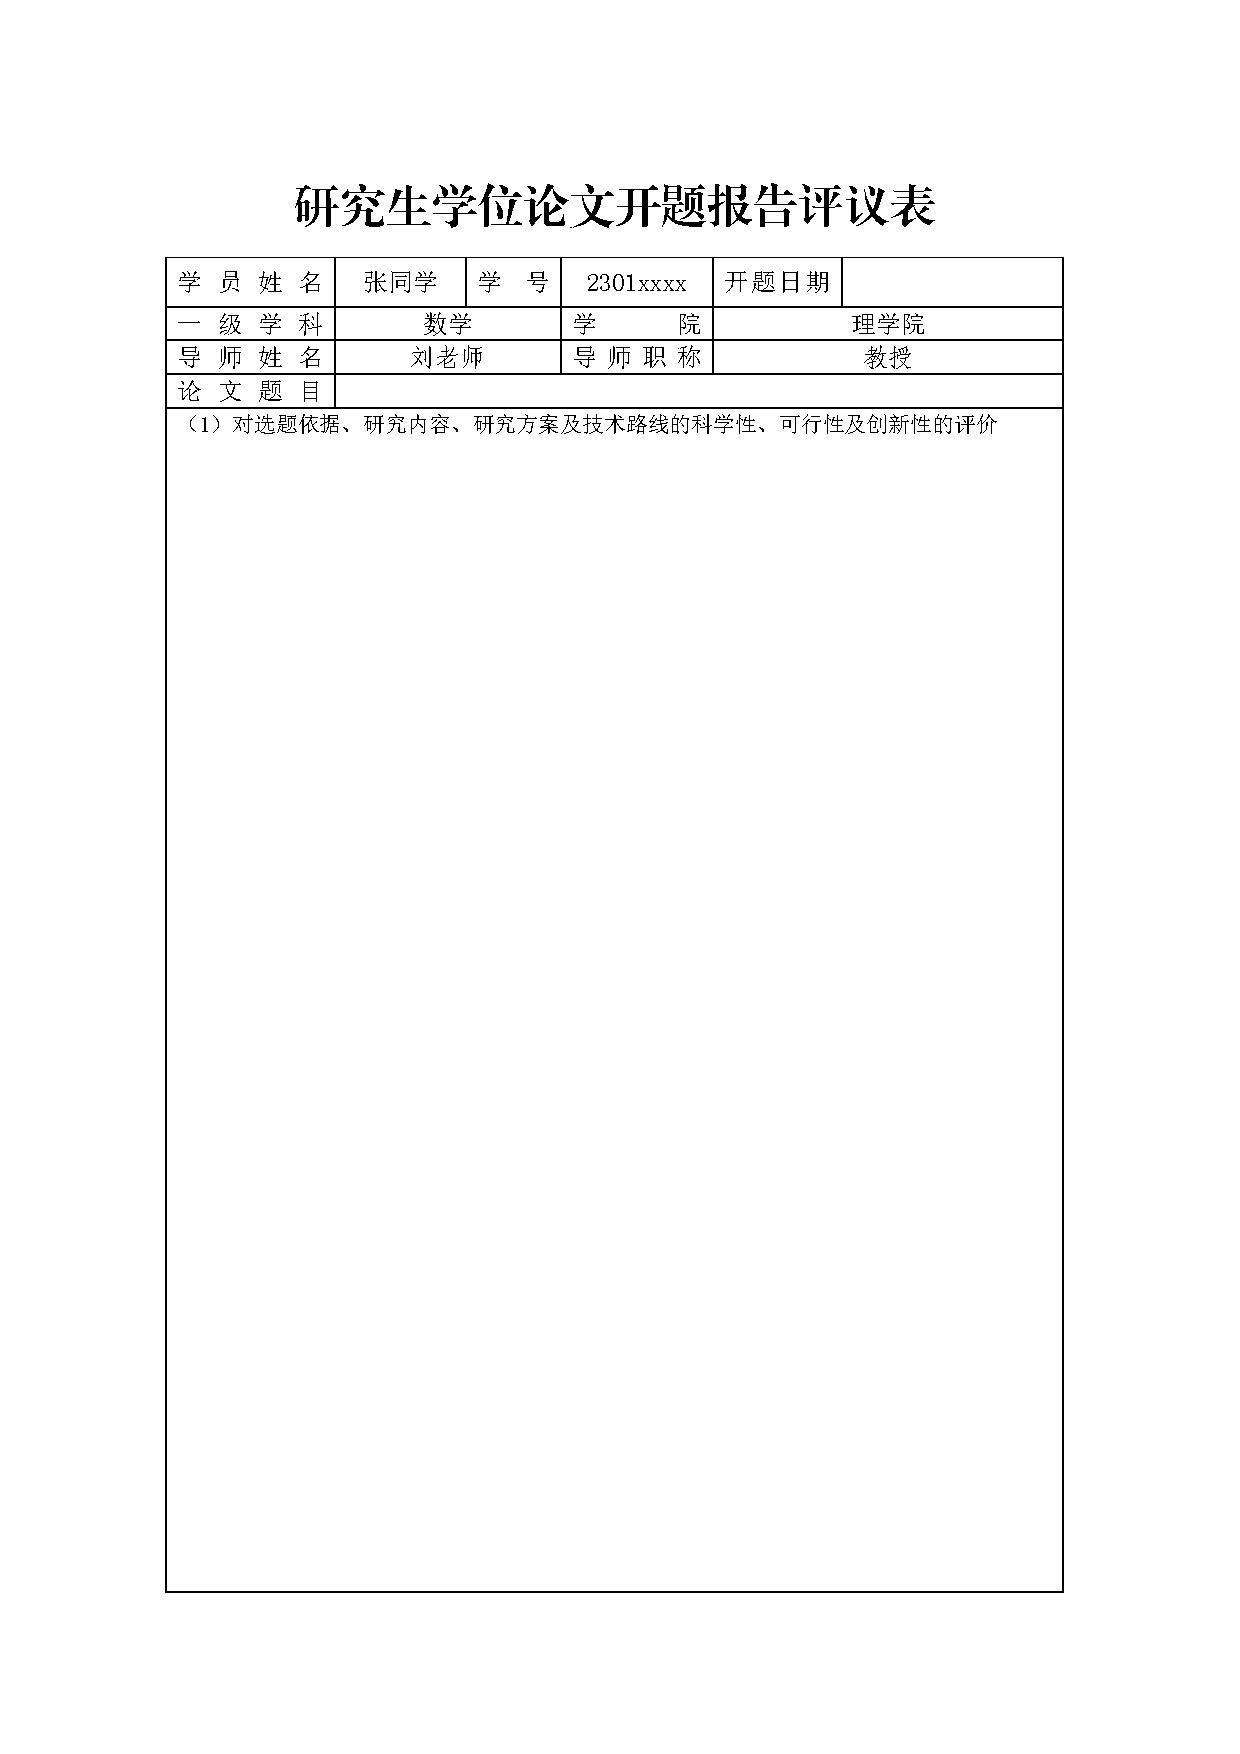
\includepdf[pages=-]{figure/研究生学位论文开题报告评议表.pdf}
\clearpage

\end{document}
